% FSDS Research Lab | Research progress report
% Compile with pdfLaTeX. Figure included in the same directory.
\documentclass[10pt,a4paper]{article}
\usepackage[T1]{fontenc}
\usepackage[utf8]{inputenc}
\usepackage[margin=2.15cm,top=3.05cm,bottom=1.9cm,headheight=1.3cm,headsep=0.45cm]{geometry}
\usepackage{xcolor,graphicx,booktabs,tabularx,array,enumitem,caption,fancyhdr,lastpage,pdflscape,float,hyperref,amssymb,amsmath,multicol,needspace,tikz}
\usetikzlibrary{positioning,arrows.meta}
\usepackage{microtype}
\usepackage{titlesec}
\definecolor{fsds}{HTML}{E8402F}
\definecolor{navy}{HTML}{1C2B47}
\definecolor{soft}{HTML}{606A7C}
\definecolor{line}{HTML}{D8DCE3}
\hypersetup{colorlinks=true,linkcolor=navy,citecolor=fsds,urlcolor=fsds,pdfauthor={Mai Anh Pham},pdftitle={FSDS Research Progress Report - Cross-Lingual Multi-Hop Unlearning}}
\pagestyle{fancy}
\fancyhf{}
\lhead{\small\textbf{FSDS Research Lab}\\\textcolor{soft}{Research Progress Report}}
\rhead{\small\textbf{Mai Anh Pham}\\\textcolor{soft}{22 October--4 November 2026}}
\renewcommand{\headrulewidth}{0.4pt}
\lfoot{\small\textcolor{soft}{Cross-Lingual Multi-Hop Machine Unlearning}}
\rfoot{\small\thepage/\pageref{LastPage}}
\renewcommand{\footrulewidth}{0pt}
\titleformat{\section}{\large\bfseries\color{navy}}{\thesection}{0.65em}{}
\titleformat{\subsection}{\normalsize\bfseries\color{navy}}{\thesubsection}{0.6em}{}
\titlespacing*{\section}{0pt}{12pt}{5pt}
\titlespacing*{\subsection}{0pt}{8pt}{3pt}
\setlength{\parindent}{0pt}
\setlength{\parskip}{4pt}
\setlist[itemize]{topsep=2pt,itemsep=2pt,leftmargin=1.3em}
\setlist[enumerate]{topsep=2pt,itemsep=3pt,leftmargin=1.55em}
\renewcommand{\arraystretch}{1.17}
\captionsetup{font=small,labelfont=bf}
\urlstyle{same}
% Unfilled supervisor names are left as editable placeholders.
\newcommand{\supervisor}{\textit{To be confirmed}}
\newcommand{\cosupervisora}{\textit{To be confirmed}}
\newcommand{\cosupervisorb}{\textit{To be confirmed}}
\newcommand{\guide}[1]{} % Template guidance is not printed.
\begin{document}

\begin{center}
{\LARGE\color{fsds}\bfseries FSDS Research Progress Report}\\[5pt]
{\Large\bfseries Cross-Lingual Multi-Hop Machine Unlearning}\\[7pt]
{\small\textbf{Researcher:} Mai Anh Pham \quad\textbar\quad \textbf{Report:} 01 \quad\textbar\quad \textbf{Period:} 22 October--4 November 2026}\\[3pt]
{\small\textbf{Stage:} v4 exploratory run complete; v5.1 full training release blocked after candidate review; no v5.1 training run}\\[4pt]
{\small\href{https://github.com/aCoderChild/fsds}{github.com/aCoderChild/fsds}}
\end{center}
\vspace{2pt}\hrule\vspace{5pt}

\section{Research Problem and Motivation}

\textbf{Subfield:} Cross-lingual Transfer of Machine Unlearning in Multi-hop Question Answering.

\textbf{Main idea:} I investigate whether unlearning an intermediate factual relationship using English-only data affects the model's ability to answer related multi-hop questions in other languages: French, German, Hindi, and Thai. I distinguish direct recall of the targeted relationship from the ability to reach its downstream final answer. This distinction is motivated by prior work on knowledge-edit propagation and multilingual forgetting \cite{zhong2023mquake,xiang2026multilingual}.

\textbf{Research goal:} An empirical evaluation of cross-lingual downstream forgetting, subject to verifying that the model learned the relevant facts and that the final answers depend on the targeted relationships \cite{waseem2026falsepositive,yang2025socrates}.

\section{Research Question and Hypothesis}

\textbf{Research question.} After a model has learned the target first-hop fact, does unlearning it with English-only examples change final-answer accuracy on dependent two-hop questions in French, German, Hindi, and Thai? Is each target-language change different from English, and is it selective relative to unrelated retain facts?

\begin{figure}[htbp]
    \centering
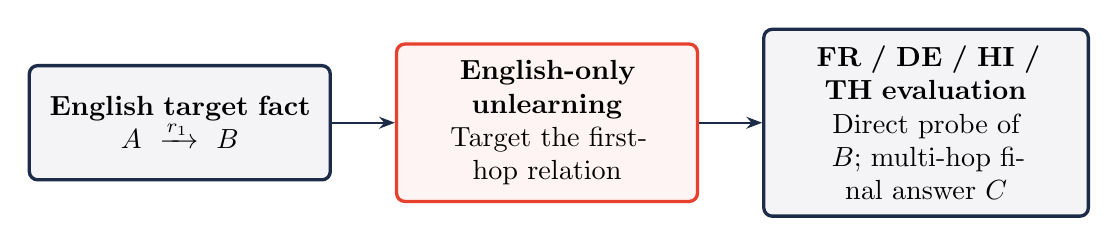
\begin{tikzpicture}[
    fact/.style={draw=navy,fill=navy!5,rounded corners=3pt,very thick,
                 align=center,text width=3.4cm,minimum height=1.45cm,inner sep=6pt},
    update/.style={draw=fsds,fill=fsds!6,rounded corners=3pt,very thick,
                   align=center,text width=3.4cm,minimum height=1.45cm,inner sep=6pt},
    eval/.style={draw=navy,fill=navy!5,rounded corners=3pt,very thick,
                 align=center,text width=3.7cm,minimum height=1.45cm,inner sep=6pt},
    flow/.style={-{Stealth[length=2mm]},line width=0.8pt,navy}
]
  \node[fact] (target) {\textbf{English target fact}\\$A \xrightarrow{r_1} B$};
  \node[update,right=0.8cm of target] (forget) {\textbf{English-only unlearning}\\Target the first-hop relation};
  \node[eval,right=0.8cm of forget] (probe) {\textbf{FR / DE / HI / TH evaluation}\\Direct probe of $B$; multi-hop final answer $C$};
  \draw[flow] (target) -- (forget);
  \draw[flow] (forget) -- (probe);
\end{tikzpicture}
    \caption{Research intuition: target the relationship $A\!\rightarrow\!B$ using English-only unlearning, then test direct recall of $B$ and the downstream answer $C$ in other languages. A correct final answer alone does not prove recovery of $B$ \cite{yang2025socrates}.}
    \label{fig:multihop_unlearning}
\end{figure}

\textbf{Hypothesis.} English-only unlearning may reduce direct recall of the target fact in non-English queries. Its effect on dependent two-hop final answers may differ by language and may be smaller or larger than the English effect. Direct-fact loss and final-answer loss are separate outcomes; the current frozen cohort supports only two-hop evaluation, so this study cannot test variation by reasoning depth \cite{xiang2026multilingual,qian2026leak}.


\section{Literature Review}

\subsection{Cross-lingual Machine Unlearning}

Xiang et al. \cite{xiang2026multilingual} investigate
whether knowledge unlearned in one language remains
accessible in other languages. Their findings show that
cross-lingual unlearning transfer varies considerably
across languages and that some forgotten knowledge can
be recovered.

Similarly, Waseem and Fawaz
\cite{waseem2026falsepositive} demonstrate that
cross-lingual forgetting can be misinterpreted when
the model never learned the target knowledge in the
evaluation language. They emphasize the importance
of comparing the base model, the fine-tuned model,
and the unlearned model, while also controlling
for general performance degradation.

These studies establish that \textbf{cross-lingual forgetting is variable and needs pre-learning controls} \cite{xiang2026multilingual,waseem2026falsepositive}. However, they do not
directly establish how forgetting an intermediate
fact affects the final answer of a multi-hop
reasoning question in another language.

\subsection{Multi-hop Reasoning and Knowledge Unlearning}

MQuAKE \cite{zhong2023mquake} evaluates whether
editing a factual relationship leads to the expected
changes in downstream multi-hop answers. It shows
that successfully updating an individual fact does not necessarily produce consistent changes in questions that depend on that fact.

R-TOFU \cite{yoon2025rtofu} extends unlearning
evaluation to reasoning traces and demonstrates
that information may remain in intermediate reasoning
steps even when final answers appear to be forgotten.

Qian et al. \cite{qian2026leak} further study how unlearned knowledge can remain accessible through
different multi-hop reasoning paths and recovery attacks.

These works highlight the importance of evaluating
knowledge beyond direct factual questions \cite{yoon2025rtofu,qian2026leak}. However, they do not jointly isolate the cross-lingual effects of unlearning a specific intermediate relationship on downstream multi-hop answers.

\subsection{Cross-Lingual Multi-Hop Editing and Recent Unlearning Benchmarks}

Khandelwal et al. introduce CroLin-MQuAKE for
cross-lingual multi-hop \emph{knowledge editing}
\cite{khandelwal2024crosslingual}. Their task is a close
methodological neighbor: an edited fact should propagate
through a multi-hop answer across languages. Editing
inserts or changes a fact, whereas the present study
tests removal of an acquired intermediate fact, so the
intervention and expected answer behavior differ.

Recent multilingual-unlearning benchmarks also narrow
the gap. $\mu^2$-Bench evaluates memorization,
unlearning, and knowledge accessibility across training
and held-out languages using synthetic profile QA
\cite{hwang2026mu2bench}. CLLPU studies whether
unlearning propagates within or beyond an intended
language boundary and includes core questions and
surface variants across ten languages
\cite{shao2026cllpu}. These benchmarks strengthen the
case for multilingual controls and carefully verified
translations. Their described evaluations focus on
knowledge-unit QA and cross-lingual accessibility; they
do not appear to test whether removal of one intermediate
edge changes the final answer of a dependent multi-hop
chain in another language. This comparison is based on
the published benchmark protocols, not a systematic
survey of every related paper.

\subsection{Controlled Knowledge and Reasoning Shortcuts}

TOFU \cite{maini2024tofu} introduces fictional author profiles to study machine unlearning under more controlled conditions. Using fictional knowledge reduces interference from information that a model may already have learned during pretraining.

However, fictional data alone does not guarantee that a model actually performs multi-hop reasoning. The model may memorize an association between the starting entity and the final answer.

SOCRATES \cite{yang2025socrates} addresses this problem by constructing multi-hop questions that reduce opportunities for shortcut-based answering. CLUTRR \cite{sinha2019clutrr} also provides controlled relational reasoning tasks that test generalization to unseen combinations of relations.

These studies motivate using controlled facts and shortcut-aware questions to test whether final answers actually depend on the intended intermediate relationships \cite{yang2025socrates,sinha2019clutrr}.

\subsection{Research Gap}

Existing research now covers cross-lingual unlearning,
cross-lingual multi-hop editing, multi-hop knowledge
leakage, and shortcut-aware reasoning evaluation. The
narrower question here is whether \emph{English-only
removal of an acquired intermediate relationship} changes
the downstream final answer to a dependent multi-hop
question asked in another language. The design measures
direct intermediate-fact recall and final-answer accuracy
separately, and compares matched cases before and after
unlearning. It also controls for prior knowledge,
incomplete SFT acquisition, reasoning shortcuts, and
collateral damage on retained facts
\cite{waseem2026falsepositive,thaker2025weak}.


\section{Experiment Design}


\subsection{Datasets}

I plan to use SynthWorlds-SM, the synthetic-mapped
version of SynthWorlds, which provides a corpus of
synthetic entities and relationships alongside
existing multi-hop question-answering tasks
\cite{gu2026synthworlds}. The dataset is designed
to distinguish reasoning performance from advantages
due to pretrained world knowledge.

Dataset:
\href{https://huggingface.co/datasets/kenqgu/SynthWorlds}
{SynthWorlds on Hugging Face}.


\begin{enumerate}
    \item \textbf{Dataset preparation:}
    Reuse SynthWorlds-SM factual triples and multi-hop
    questions without inventing new facts \cite{gu2026synthworlds}.
    Audit whether every selected target relationship lies
    on a valid dependency path to its final answer.

    \item \textbf{Translation:}
    Translate the selected factual and evaluation questions into
    English (EN), French (FR), German (DE), Hindi (HI), and Thai (TH),
    preserving entity identifiers, relation direction, and answer type.
    In the v5.1 feasibility pilot, translation screening is AI-only and
    hash-bound; it is not fluent-human certification. The target answer
    remains the canonical entity name across languages. Thus the pilot
    measures answering multilingual-input questions with the correct
    entity, not the fluency of generated answer prose in each language.

    \item \textbf{Dataset splitting:}
    Split by factual chain or connected entity group into
    forget, retain, and holdout sets to prevent leakage.

    \item \textbf{Knowledge acquisition:}
    Fine-tune the model on factual relationships
    in all five languages using SFT.

    \item \textbf{Pre-unlearning verification:}
    Verify direct factual recall and multi-hop
    final-answer accuracy in each language.

    \item \textbf{English-only unlearning:}
    Unlearn selected intermediate factual relationships using English-only data.

    \item \textbf{Cross-lingual evaluation:}
    Compare multi-hop final-answer accuracy before and after unlearning across all five languages.
\end{enumerate}


\subsection{Models and Knowledge Acquisition}

\begin{enumerate}
    \item \textbf{Model selection:}
    Use Llama 3.2 1B-Instruct for the feasibility pilot
    and Llama 3.1 8B-Instruct for the main study
    \cite{meta2024llama32,meta2024llama31}.

    \item \textbf{Motivation:}
    Test whether language-dependent model competence is
    associated with English-only forgetting transfer.
    Meta lists all five study languages among Llama 3.1's
    supported languages \cite{meta2024llama31}.

    \item \textbf{Knowledge acquisition:}
    Use supervised fine-tuning (SFT) on factual question-answer
    pairs and disjoint composition practice from SynthWorlds-SM in five languages:
    English (EN), French (FR), German (DE),
    Hindi (HI), and Thai (TH).

    \item \textbf{Reasoning preparation:}
    Exclude evaluation multi-hop QA pairs and direct
    start-to-final-answer shortcuts from factual SFT.
    Train composition practice only on disjoint chains
    \cite{yang2025socrates,sinha2019clutrr}.
\end{enumerate}

\subsection{Pre-Unlearning Verification}

\begin{enumerate}
    \item \textbf{Baseline evaluation:}
    Evaluate the pretrained model to identify
    any existing factual knowledge.

    \item \textbf{Knowledge verification:}
    After SFT, evaluate the model in all five
    languages using:
    \begin{itemize}
        \item Direct factual recall.
        \item Multi-hop final-answer accuracy.
        \item A direct-positive probe, a direct-negative control,
        and a two-hop final-answer probe. The frozen v5.1
        evaluation has one wording per probe, case, and language;
        it does not test paraphrase robustness or compare multiple
        hop depths.
    \end{itemize}

    \item \textbf{Case selection:}
    Identify factual chains answered correctly
    before unlearning and record eligible cases
    for each language in the fixed two-hop setting.

    \item \textbf{Evaluation control:}
    Compare pre- and post-unlearning performance
    on the same cases to avoid treating
    unlearned knowledge as forgotten knowledge
    \cite{waseem2026falsepositive}.
\end{enumerate}

\subsection{English-Only Unlearning}

\begin{enumerate}
    \item \textbf{Unlearning target:}
    Target the first factual relationship in selected
    multi-hop chains using English-only QA pairs.

    \item \textbf{Unlearning methods:}
    Compare three methods:
    \begin{itemize}
        \item Gradient Ascent (GA).
        \item Gradient Difference (GD).
        \item Negative Preference Optimization (NPO)
        \cite{zhang2024npo}.
    \end{itemize}

    \item \textbf{Reference models:}
    Compare with pretrained, full-SFT, and retain-only
    checkpoints to distinguish forgetting from weak
    acquisition and general degradation
    \cite{waseem2026falsepositive,maini2024tofu}.

    \item \textbf{Utility preservation:}
    Monitor retain-set accuracy and generation quality
    to distinguish targeted forgetting from
    general model degradation
    \cite{zhang2024npo,thaker2025weak}.
\end{enumerate}


\subsection{Cross-Lingual Multi-hop Evaluation}

\begin{enumerate}
    \item \textbf{Evaluation languages:}
    English (EN), French (FR), German (DE),
    Hindi (HI), and Thai (TH).

    \item \textbf{Evaluation metrics:}
    \begin{itemize}
        \item \textbf{Direct recall:}
        Accuracy on targeted intermediate facts.

        \item \textbf{Multi-hop accuracy:}
        Accuracy of final answers to multi-hop questions
        involving the targeted facts (primary metric).

        \item \textbf{Knowledge retention:}
        Accuracy on unrelated factual chains.
    \end{itemize}

    \item \textbf{Cross-lingual transfer:}
    Compare pre- and post-unlearning accuracy
    on matched factual chains in each language.

    \item \textbf{Selectivity:}
    Compare changes in forget-set and retain-set
    performance to identify unintended degradation
    \cite{maini2024tofu,thaker2025weak}.
\end{enumerate}


\subsection{Controlling for Reasoning Shortcuts}

\begin{enumerate}
    \item \textbf{Prevent answer memorization:}
    Exclude exact evaluation multi-hop QA pairs
    from SFT.

    \item \textbf{Shortcut detection:}
    Check for direct associations between
    starting entities and final answers.

    \item \textbf{Dependency verification:}
    Where supported by the dataset, test alternative
    questions or factual paths using existing
    verified relationships
    \cite{zhong2023mquake,yang2025socrates}.

    \item \textbf{Interpretation:}
    Distinguish correct downstream answers from
    verified recovery of intermediate knowledge.
\end{enumerate}



\subsection{Analysis Plan}

I will evaluate whether English-only unlearning of
intermediate factual relationships affects multi-hop
question answering across five languages: English (EN),
French (FR), German (DE), Hindi (HI), and Thai (TH).

The primary estimand is the absolute post-minus-pre change
in target-language multi-hop exact match, reported for each
language and each of the three unlearning methods. The
primary family therefore contains 12 planned method-language
cells; none will be selected after seeing the results. Each
cell uses the same forget cases that were competent on both
the direct and multi-hop probes in English and that target
language before unlearning. Entity groups are resampled as
clusters, and two-sided 95\% intervals are Bonferroni-adjusted
over these 12 cells. I will show the three seed-specific
estimates as well as their equal-weight mean; the intervals
condition on the three observed seeds and do not establish
precision over all training randomness.

The paired target-minus-English difference-in-differences
(DID) is the key secondary estimand: it asks whether a target
language's change differs from English, not whether the target
language changed at all. I will report both component changes
on exactly the same bilingual precompetent cases and give the
12 planned DID cells their own Bonferroni-adjusted 95\%
interval family. Retain-set changes remain a separate
utility/selectivity check. The 15-case/8-group threshold is a
feasibility gate, not a power calculation; no confirmatory
claim will be made from a run that fails it.

\subsubsection*{Evaluation Metrics}

\begin{enumerate}

    \item \textbf{Pre-unlearning competence:}
    Measure direct factual recall and multi-hop
    final-answer accuracy after SFT. Record cases
    answered correctly before unlearning
    \cite{waseem2026falsepositive}.

    \item \textbf{Direct forgetting:}
    Measure the reduction in recall of targeted
    intermediate facts across languages
    \cite{xiang2026multilingual}.

    \item \textbf{Target-language multi-hop change (primary outcome):}
    Measure post-minus-pre final-answer accuracy for each
    target language on forget cases that were competent in
    English and that target language before unlearning.
    This is the outcome that directly answers whether
    non-English performance changed.

    \item \textbf{Differential cross-language effect (key secondary contrast):}
    On those same cases, compare the target-language
    change with the English change. This indicates whether
    the effect differs from English; it is not a substitute
    for the absolute target-language change \cite{zhong2023mquake}.

    \item \textbf{Downstream answer persistence:}
    Measure how often the final answer remains
    correct when direct recall of the targeted
    intermediate fact fails. This is a proposed
    case-level metric; it is not evidence of
    recovered reasoning traces \cite{yang2025socrates}.

    \item \textbf{Knowledge retention:}
    Measure accuracy on unrelated factual chains
    before and after unlearning
    \cite{maini2024tofu}.

    \item \textbf{Cross-lingual persistence:}
    Consider the Knowledge Persistence Score (KPS)
    for consistency of forgetting across language
    pairs, using the original definition of
    Hwang et al. \cite{hwang2026knowledge}.

    \item \textbf{Reliability and validity:}
    Compare methods across languages and hop depths.
    Report generation failures, repeated seeds, and
    paired confidence intervals. Examine possible
    reasoning shortcuts \cite{yang2025socrates}.

\end{enumerate}

\subsubsection*{Metric Definitions}

Let $\mathrm{Acc}_{\mathrm{pre}}$ and
$\mathrm{Acc}_{\mathrm{post}}$ denote accuracy before
and after unlearning.

For target language $\ell$, the absolute change on the
pre-unlearning bilingual-competent forget set is:

\[
\Delta_{\ell,F} =
\mathrm{Acc}_{\mathrm{post,MH},\ell,F}
-
\mathrm{Acc}_{\mathrm{pre,MH},\ell,F}.
\]

A negative value indicates reduced downstream
multi-hop performance in language $\ell$.

The primary cross-language contrast uses cases that are
pre-unlearning competent in both English and the target
language. For case $i$ and target language $\ell$, define:

\[
\mathrm{DID}_{i,\ell} =
\left(C_{\mathrm{post},i,\ell} - C_{\mathrm{pre},i,\ell}\right)
-
\left(C_{\mathrm{post},i,\mathrm{EN}} - C_{\mathrm{pre},i,\mathrm{EN}}\right).
\]

The paired DID estimate is the mean contrast across cases,
with entity groups resampled as clusters and seed variation
reported separately. The primary target-language changes
and secondary DID intervals use a two-sided Bonferroni
adjustment across their respective 12 method-language cells.
Its components, $\Delta_{\ell,F}$ and
$\Delta_{\mathrm{EN},F}$, are calculated on the same cases
and reported with their own cluster-bootstrap intervals.
A negative DID means target-language accuracy declined
more than English accuracy. The absolute target-language
change remains the direct answer to whether that language's
accuracy changed.

Direct forgetting is measured as:

\[
F_{\mathrm{direct}} =
\mathrm{Acc}_{\mathrm{pre,direct}}
-
\mathrm{Acc}_{\mathrm{post,direct}}.
\]

A positive value indicates reduced direct recall.

For downstream answer persistence, let $B$ denote
the targeted intermediate fact and $C$ the
multi-hop final answer.

For each language and split, first restrict to cases
where full SFT answered both the direct and multi-hop
probes correctly. Within that pre-unlearning competent
set, I will calculate:

\[
\mathrm{DAP} =
\frac{
N(B_{\mathrm{pre}}=\mathrm{correct},
  C_{\mathrm{pre}}=\mathrm{correct},
  B_{\mathrm{post}}=\mathrm{wrong},
  C_{\mathrm{post}}=\mathrm{correct})
}{
N(B_{\mathrm{pre}}=\mathrm{correct},
  C_{\mathrm{pre}}=\mathrm{correct},
  B_{\mathrm{post}}=\mathrm{wrong})
}.
\]

DAP measures the proportion of direct-recall failures
for which the downstream answer remains correct.
It does not establish recovery of the intermediate
fact. If no direct-recall failures occur, DAP is
undefined and will be reported as N/A.

KPS, if reported, will follow its published definition
\cite{hwang2026knowledge} and will not be conflated
with the proposed downstream answer persistence metric.

\subsubsection*{Proposed Results Tables}

\textbf{Pre-unlearning Knowledge Verification}

\begin{table}[htbp]
\centering
\small
\setlength{\tabcolsep}{4pt}

\begin{tabularx}{\linewidth}{@{}Xrrrr@{}}
\toprule
\textbf{Language} &
\textbf{Total} &
\textbf{Direct (\%)} &
\textbf{MH (\%)} &
\textbf{Eligible} \\
\midrule
\multicolumn{5}{c}{Not run: the v5.1 training release is blocked before SFT.} \\
\bottomrule
\end{tabularx}

\caption{
Pre-unlearning factual recall and multi-hop
(MH) accuracy after SFT. Eligible cases
are those answered correctly on both tasks
before unlearning.
}
\label{tab:baseline}
\end{table}

No v5.1 model predictions or eligible case counts
are available yet. The historical v4 exploratory
results below are reported separately and must not
be substituted into this table.

Full-set results and eligible-case results will be
reported separately to distinguish forgetting from
incomplete knowledge acquisition.


\textbf{Main Cross-Lingual Unlearning Results}

\begin{table}[H]
\centering
\scriptsize
\setlength{\tabcolsep}{3pt}
\renewcommand{\arraystretch}{1.15}

\begin{tabularx}{\linewidth}{@{}llrrrrr@{}}
\toprule
\textbf{Method} &
\textbf{Lang.} &
\textbf{N} &
\textbf{Direct} &
\textbf{MH} &
\textbf{Retain} &
\textbf{Invalid} \\
 & & &
\textbf{(\%)} &
\textbf{(\%)} &
\textbf{$\Delta$ pp} &
\textbf{(\%)} \\
\midrule

\multicolumn{7}{c}{Not run: no v5.1 baseline competence gate or unlearning results.} \\

\bottomrule
\end{tabularx}

\caption{
Post-unlearning accuracy on previously correct
forget-set cases. N is the number of eligible cases.
Direct and MH are post-unlearning accuracies.
Retain $\Delta$ is the percentage-point change
(post minus pre) on the unrelated retain set.
Invalid denotes malformed or repetitive outputs.
}
\label{tab:unlearning}
\end{table}

\textbf{Primary Target-Language Outcome and Secondary DID}

\begin{table}[H]
\centering
\scriptsize
\setlength{\tabcolsep}{4pt}
\renewcommand{\arraystretch}{1.15}

\begin{tabularx}{\linewidth}{@{}llrrrrrX@{}}
\toprule
\textbf{Method} &
\textbf{Language} &
\textbf{Cases} &
\textbf{Groups} &
\textbf{EN $\Delta$ (pp)} &
\textbf{Target $\Delta$ (pp)} &
\textbf{DID (pp)} &
\textbf{Paired group-bootstrap 95\% CI} \\
\midrule
\multicolumn{8}{c}{Not run: the v5.1 release and baseline competence gates have not passed.} \\
\bottomrule
\end{tabularx}

\caption{Planned paired effects, averaged equally across the three matched seeds. The primary outcome is target-language post-minus-pre multi-hop exact-match change; the target-minus-English difference-in-differences (DID) is secondary. The table is intentionally empty until the v5.1 release and baseline competence gates pass.}
\label{tab:primary_did}
\end{table}


\Needspace{20\baselineskip}

\textbf{Intermediate-Fact and Final-Answer Outcomes}

\begin{table}[H]
\centering
\scriptsize
\setlength{\tabcolsep}{3pt}
\renewcommand{\arraystretch}{1.15}

\begin{tabularx}{\linewidth}{@{}llrrrr@{}}
\toprule
\textbf{Method} &
\textbf{Lang.} &
\textbf{B fail} &
\textbf{B fail} &
\textbf{B pass} &
\textbf{B pass} \\
 & &
\textbf{C pass} &
\textbf{C fail} &
\textbf{C pass} &
\textbf{C fail} \\
\midrule

\multicolumn{6}{c}{Not run: paired post-unlearning outcomes are unavailable for v5.1.} \\

\bottomrule
\end{tabularx}

\caption{
Paired direct and multi-hop outcomes after unlearning.
B denotes the targeted intermediate fact and C the
final answer. Each cell reports the percentage of
eligible cases. The four outcomes sum to 100\%
within each method-language group.
}
\label{tab:persistence}
\end{table}

The main outcome of interest is
\textbf{B fail, C pass}, where direct factual
recall fails but the downstream answer remains correct.

I will distinguish this outcome from verified
recovery of intermediate knowledge.


\textbf{Effect of Reasoning Depth}

\begin{table}[htbp]
\centering
\small
\setlength{\tabcolsep}{4pt}

\begin{tabularx}{\linewidth}{@{}Xlrrr@{}}
\toprule
\textbf{Method} &
\textbf{Language} &
\textbf{2-hop} &
\textbf{3-hop} &
\textbf{4-hop} \\
\midrule

\multicolumn{5}{c}{Not run: the release and competence gates have not passed.} \\

\bottomrule
\end{tabularx}

\caption{
Change in multi-hop final-answer accuracy
($\Delta_{\mathrm{MH}}$, percentage points)
after English-only unlearning, grouped
by language and reasoning depth.
Results are reported only for hop depths
supported by sufficient eligible cases.
}
\label{tab:hop_depth}
\end{table}

\Needspace{5\baselineskip}

The frozen v5.1 evaluation cohort contains 80 Type-A cases, each with exactly two relation edges. No v5.1 baseline or unlearning result is currently estimable because the training release and competence gates have not passed. Even after those gates, this cohort can estimate only the 2-hop column; it contains no 3-hop or 4-hop cases, so those depths are not represented, not zero effects.


\subsubsection*{Statistical Analysis}

\begin{enumerate}

    \item Repeat unlearning experiments using
    at least three random seeds.

    \item Report mean accuracy and standard deviation
    across seeds.

    \item Calculate paired 95\% bootstrap confidence
    intervals over factual chains, preserving
    matched case identities before and after
    unlearning.

    \item Compare changes between forget and retain
    sets to assess selective forgetting.

    \item Compare outcomes across languages,
    reasoning depths, and unlearning methods.

    \item Treat the 15-case/8-group competence threshold
    as a feasibility gate, not a power analysis. Before
    confirmatory claims, establish the required sample size
    from a pre-specified meaningful effect and cluster-aware
    power analysis.

    \item Inspect incorrect, malformed, and repetitive
    responses to identify generation collapse
    and possible reasoning shortcuts.

\end{enumerate}

The main analysis will ask whether changes in direct recall of the targeted intermediate fact accompany downstream multi-hop accuracy changes in other languages, without comparable degradation on unrelated factual chains \cite{thaker2025weak}.


\subsection*{Feasibility-pilot result (2026-11-02)}

The evaluation-disjoint SynthWorlds-SM pilot completed five-language LoRA SFT and a baseline-only evaluation in the Kaggle Notebook Editor using Llama 3.2 1B-Instruct. The SFT used 1,655 rows (331 per language): 765 forget-split atomic-fact rows, 390 retain-split rows, and 500 rows from 50 additional training-only chains. The retain-only reference used 890 retain and training-only rows. Both runs used three epochs and seed 42. The 129 evaluation chains were grouped into 77 forget, 26 retain, and 26 holdout cases.

On the forget split, SFT direct-recall and multi-hop exact-match accuracy were:

\begin{center}
\begin{tabular}{lccccc}
\toprule
 & EN & FR & DE & HI & TH \\
\midrule
Direct recall (\%) & 88.3 & 84.4 & 77.9 & 83.1 & 83.1 \\
Multi-hop answer (\%) & 10.4 & 9.1 & 18.2 & 14.3 & 15.6 \\
\bottomrule
\end{tabular}
\end{center}

The evaluator produced 3,870 predictions across the pretrained, full-SFT, and retain-only checkpoints; it recorded zero generation failures and zero output-invalid flags. The holdout accuracy was zero because its facts were excluded from training; this is a split-control result, not evidence of forgetting. Retain results overlap retain-composition training and are training-overlap controls.

Only eight of the 77 English forget cases were SFT-precompetent on both direct and multi-hop probes. The paired English-plus-language counts were FR 2 cases/2 entity groups, DE 4/3, HI 4/3, and TH 3/3. Each language falls below the predeclared pilot feasibility floor of 15 cases and 8 groups. At that point, the baseline gate blocked the standard unlearning path and post-unlearning evaluation. The exploratory override run on 2026-11-03 is reported separately below. The baseline alone does not answer the cross-language unlearning hypothesis. Translations were reviewed AI-only; fluent human review was not performed. The exact forget multi-hop prompts were excluded from SFT, but their atomic supporting facts were included, so this tests held-out composition prompts over trained facts rather than unseen-fact generalization.

\subsection*{Follow-up diagnostic update (2026-11-03)}

The v4 composition corpus increased five-language SFT to 3,355 rows (671 per language), adding 85 source-verified Type-B training-only chains. Kaggle run manifests record completion of full SFT, a retain-only reference, and baseline evaluation on the same frozen 129-case evaluation set. The baseline evaluation covered 3,870 predictions; the exploratory post-unlearning evaluation covered 7,740. Both archives report zero generation failures and zero deterministic output-invalid flags. Archive hashes and row counts were verified, and rescoring the saved predictions with the current evaluator reproduced the scored predictions, summaries, and contrast files byte-for-byte.

The documented bilingual-competence gate still failed. Among 77 forget cases, 15 were English SFT-precompetent under the direct-plus-full-multi-hop selection rule. Matched English/non-English precompetent cases and leakage-isolated groups were FR 10/6, DE 9/5, HI 9/6, and TH 11/7; the floor was 15 cases and 8 groups for each language. An explicitly labeled exploratory override then ran GA, GD, and NPO on the 15 English first-hop forget rows, with no holdout rows. This one-seed 1B diagnostic is not a result from the planned main study.

Under the current analysis plan, the primary outcome is the absolute target-language post-minus-pre change. For GA, GD, and NPO, the pilot estimates were FR $0.0$ pp, DE $-11.1$ pp, HI $-11.1$ pp, and TH $-18.2$ pp. Separately Bonferroni-adjusted nominal 95\% intervals from fully enumerated entity-group bootstrap distributions were FR $[0.0,0.0]$, DE $[-80.0,0.0]$, HI $[-66.7,0.0]$, and TH $[-85.7,0.0]$ pp. The French interval is degenerate because no matched French case changed. These intervals condition on one seed and only 5--7 groups; full enumeration removes resampling Monte Carlo noise, not small-sample uncertainty.

The following table reports the secondary target-language-minus-English difference-in-differences (DID), in percentage points. Intervals are separately Bonferroni-adjusted over the 12 method-language cells:

\begin{center}
\small
\begin{tabularx}{\textwidth}{@{}l c X X X@{}}
\toprule
Language & Cases/groups & GA & GD & NPO \\
\midrule
FR & 10/6 & +10.0 [0.0, 66.7] & +10.0 [0.0, 66.7] & +10.0 [0.0, 66.7] \\
DE & 9/5 & +22.2 [0.0, 100.0] & +11.1 [-60.0, 100.0] & +11.1 [-60.0, 100.0] \\
HI & 9/6 & 0.0 [-66.7, 66.7] & +11.1 [0.0, 66.7] & +11.1 [0.0, 66.7] \\
TH & 11/7 & +9.1 [-42.9, 71.4] & +9.1 [-71.4, 100.0] & +9.1 [-42.9, 71.4] \\
\bottomrule
\end{tabularx}
\end{center}

All 12 primary and 12 secondary familywise intervals include or touch zero. These wide, low-cluster-count intervals do not establish that cross-language transfer is absent. Full tables, code, hashes, and limitations are in the reliability tracker at \url{reports/hypothesis_diagnostics/r1_reliability_tracker_2026-11-05/}.

The initial GD/NPO run used only 15 of 26 available English retain rows because its sampler restarted each epoch; those outputs are retained as historical audit artifacts. The sampler was corrected to cycle through every retain row before reuse, and GD/NPO were rerun in the interactive Kaggle Notebook Editor session. The corrected manifests record 26 unique retain rows per method, 15 English forget rows, zero holdout rows, and 45 optimizer steps. GA has no retain regularizer; its adapter was reused after a hash match. The corrected evaluation contains 7,740 unique prediction keys (1,290 per model across six checkpoints), with zero generation failures and zero deterministic output-invalid flags.

This is still a one-seed, 1B-model exploratory diagnostic. The documented competence floor is unmet, and translations received AI-only review without fluent-human review. The run manifests omit the unlearning-script hash, so the bundled source and outputs were reconciled after the run rather than cryptographically linked. A separate local V3 snapshot check flags one changed working-notebook hash (182/183 listed files match); the archived run scores reproduce, but historical notebook-to-run association remains incomplete. Training and evaluation used the interactive Notebook Editor because the Kaggle API-launched route did not receive notebook secrets. The V3 archive passed CRC and all indexed SHA-256 checks; its artifacts and local verification record are at \url{reports/hypothesis_diagnostics/r1_synthworlds_v4_retainfix_corrected_2026-11-03/}.

As an exploratory sensitivity check, I also subtracted the corresponding target-language-minus-English change on the retain split from the forget-split contrast. This adjusts for language-specific drift on non-forgotten examples; it is not a replacement for the primary estimand. Forget and retain entity groups were independently resampled. The analysis uses the same bilingual precompetence rule and 10,000 cluster-bootstrap draws:

\begin{center}
\scriptsize
\begin{tabularx}{\textwidth}{@{}lrrXXX@{}}
\toprule
Language & Forget cases/groups & Retain cases/groups & GA adjusted (95\% CI, pp) & GD adjusted (95\% CI, pp) & NPO adjusted (95\% CI, pp) \\
\midrule
FR & 10/6 & 21/17 & $+5.2\,[-22.2,45.3]$ & $+5.2\,[-17.8,44.9]$ & $+5.2\,[-18.9,43.3]$ \\
DE & 9/5 & 21/17 & $+27.0\,[-0.7,89.5]$ & $+6.3\,[-40.0,74.1]$ & $+6.3\,[-43.5,74.1]$ \\
HI & 9/6 & 19/13 & $-5.3\,[-42.0,33.3]$ & $+5.8\,[-8.7,44.4]$ & $+5.8\,[-8.7,44.4]$ \\
TH & 11/7 & 21/16 & $-0.4\,[-35.3,44.6]$ & $+4.3\,[-44.1,63.0]$ & $-0.4\,[-36.0,46.0]$ \\
\bottomrule
\end{tabularx}
\end{center}

All 12 adjusted intervals include zero and remain wide, so this sensitivity also provides no reliable language-specific effect. It is based on a small, one-seed pilot and should be treated as exploratory. The reproducible analysis script is \texttt{scripts/analyze\_retain\_adjusted\_crosslingual.py}; its input case-metrics SHA-256 and results are recorded under \path{reports/hypothesis_diagnostics/r1_synthworlds_v4_retainfix_corrected_2026-11-03/supplementary/retain_adjusted/}.

\subsection*{Source-answer cardinality audit (2026-11-03)}

A read-only audit checked the source fact inventory for all 200 Type-A questions. The 70 previously excluded Q1 questions have multiple source-supported answers, so their original open-ended direct labels are ambiguous. For every one of those 70, the graph-selected bridge is the only Q1 candidate with a source-supported R2 continuation. In 67 cases, the complete R2 answer set matches the single gold final answer; three cases have multiple source-supported final answers. Among the frozen 129 evaluation cases, 128 have a unique source-supported final-answer set. The remaining case, 0038-qa-sm, is in holdout; all 103 forget/retain cases have unique final-answer sets.

\begin{center}
\small
\begin{tabularx}{\textwidth}{@{}l r r r X@{}}
\toprule
Candidate set & Cases & Q1 unique & Q1 ambiguous & Final-answer source check \\
\midrule
All Type-A source questions & 200 & 130 & 70 & 196 match the complete source-supported answer set; 4 are multi-answer or mismatched \\
Frozen v4 evaluation & 129 & -- & -- & 128 unique; one ambiguous holdout label \\
Potential expanded cohort & 195 & -- & 67 recovered & Unique final-answer set; excludes three multi-answer paths and the 0080 source/graph conflict \\
\bottomrule
\end{tabularx}
\end{center}

The holdout label issue does not change the saved holdout score: rescoring its 30 final-answer predictions against both source-supported answers still gives zero exact matches. It does not enter the primary forget-set contrast. The cardinality audit identified a potential 195-case cohort and found an exact 117/39/39 allocation feasible under its original grouping rule. Recovering the 67 ambiguous-Q1 cases requires a fact-specific yes/no direct probe. The current v4 data and results remain frozen. Reproducible source counts and hashes are in \texttt{reports/hypothesis\_diagnostics/r1\_answer\_cardinality\_audit\_2026-11-03/}.

A separate source-to-SFT overlap audit then compared this candidate pool against the completed 3,355-row composition corpus:

\begin{center}
\small
\begin{tabularx}{\textwidth}{@{}Xr@{}}
\toprule
Overlap screen & Count \\
\midrule
Candidate Type-A questions already used as SFT train-only examples & 50 / 195 \\
Type-B train-only QA IDs sharing graph QIDs with candidate cases & 27 / 85 \\
Candidate cases with Type-B graph-QID overlap & 23 \\
Type-B train-only QA IDs with an exact candidate answer-surface match & 31 / 85 \\
Candidate groups touched by these training-only overlap screens & 28 / 104 \\
Candidate cases left after excluding all touched groups & 94 / 195 \\
\bottomrule
\end{tabularx}
\end{center}

The 117/39/39 calculation covers candidate groups only; it does not establish separation from the SFT corpus. The current checkpoint cannot be reused for the expanded cohort. Exact answer-surface and QID collisions are conservative exposure signals, not proof that each targeted relation was trained. Details and hashes are in \texttt{reports/hypothesis\_diagnostics/r1\_candidate\_sft\_overlap\_audit\_2026-11-03/}.

\subsection*{v5 cohort and direct-probe draft (2026-11-03)}

A new quarantined v5 draft applies stronger grouping than the cardinality audit: it connects shared graph/entity QIDs, source facts, normalized answers, all graph-node name surfaces, and entity aliases. This merges two same-surface entities that had different QIDs, reducing the candidate pool from 104 to 102 indivisible groups; the largest group contains 24 cases. A SciPy mixed-integer allocation assigns exactly 117 forget, 39 retain, and 39 holdout cases while balancing group counts, ambiguous-Q1 cases, and date/year-shaped final answers. The split has 61, 21, and 20 leakage groups in those sets, respectively. The source-verified candidate counts by split are 40/14/13 ambiguous-Q1 cases and 37/12/13 date/year-shaped final answers.

The draft direct probe asks whether the designated bridge is a valid answer to Q1 and requests exactly \texttt{YES} or \texttt{NO}. Each positive is paired with a source-derived entity outside the complete Q1 answer set as a negative control; 185 controls use the same relation under another subject, and 10 use another source relation under the same subject. These labels use the synthetic fact inventory as a closed-world reference. Controls do not overlap candidate entities, the old v4 train-only composition entities, or controls assigned to another split. The multi-hop prompt remains the original composed question, and its final answer is source-verified and unique for all 195 cases.

An independent verifier rechecked all 195 target fact paths, final labels, direct-control membership, source hashes, artifact hashes, and cross-split group/QID/fact/answer-surface separation. It passed. The new split, labels, and prompts remain \textbf{DRAFT\_NOT\_APPROVED}; every artifact is marked \texttt{do\_not\_train} and \texttt{do\_not\_evaluate}.

The corrected v5.1 prompt metadata now protects every source-supported entity in both target facts and the question text. The earlier v5 translation screen is superseded because it omitted some intermediate entities from its protection metadata. In v5.1, NLLB-200 distilled 600M produced machine drafts for all 2,340 rows; Qwen2.5 7B fallback recovered 102 marker failures, while three Hindi rows remained blocked for failing protected-name checks. The blinded AI-only screen accounted for every row: 2,337 reviewed, 1,721 passed, 616 were flagged, and three translations failed. There were no unresolved reviewer calls or conflicting decisions for duplicate masked pairs. Of the reviewed rows, 2,235 were cross-model checks and 102 were same-model fallback self-checks. No fluent-human review was performed.

\begin{center}
\small
\begin{tabular}{lrrrrr}
\toprule
Language & Reviewed & AI pass & Flagged & Translation failures & Pass rate \\
\midrule
French & 585 & 446 & 139 & 0 & 76.2\% \\
German & 585 & 457 & 128 & 0 & 78.1\% \\
Hindi & 582 & 414 & 168 & 3 & 70.8\% \\
Thai & 585 & 404 & 181 & 0 & 69.1\% \\
\textbf{Total} & \textbf{2,337} & \textbf{1,721} & \textbf{616} & \textbf{3} & \textbf{73.5\%} \\
\bottomrule
\end{tabular}
\end{center}

The initial screen found only 9 forget cases across 7 groups with both primary probes passing in all four target languages. A subsequent full repair and blinded-screen pass superseded that count: 2,137 of 2,340 rows passed, 156 were flagged, and 47 translation attempts failed. Its raw all-probe intersection contains 44 forget cases across 25 groups, 21 retain cases across 13 groups, and 18 holdout cases across 11 groups. The release applies a stricter independence rule and excludes three cases that relied on a same-model self-check; the frozen evaluation set therefore contains 80 cases and 1,200 prompt/label rows: 43 forget cases across 24 groups, 20 retain across 12 groups, and 17 holdout across 11 groups. These counts establish translation-screen eligibility only; model pre-unlearning competence remains unknown until the three-seed baseline is run. The current evaluation cohort and reproducible screen are in \path{experiments/synthworlds_r1/training_release_draft/evaluation/} and \path{experiments/synthworlds_r1/translation_reviews/translategemma_repair_v1_full/diagnostic_report.md}. The separate five-language training corpus is not approved, and no v5.1 SFT or unlearning run has started. All translation review is AI-only, without fluent-human certification. The completed training-question review still leaves too few complete forget and retain cases and no eligible training-only composition chains; the exact release-gate counts are reported in the current audit subsection below. The two Qwen reviewers share a model family, so their errors may be correlated.

To assess a lower-cost repair route without changing release inputs, a deterministic sample of eight flagged atomic and eight flagged composition prompts per target language (64 total) was translated with TranslateGemma 4B and screened by Qwen2.5 7B. The recorded integrity results for this earlier calibration have not been independently revalidated against the source name lists; 48 passed the recorded Qwen semantic/fluency screen (French 12/16, German 14/16, Hindi 13/16, Thai 9/16). Rejected examples included relation-direction, scope, answer-type, and fluency problems. This calibration is too small to estimate corpus-wide repair quality and approves no rows. The original translations, reviews, and manifests were not modified. The diagnostic files are in \path{experiments/synthworlds_r1/training_release_draft/translation_repair_diagnostics/translategemma4b_qwen7b_calibration64_2026-11-03/}. The training release still requires all 1,952 target-language questions and all 44 training-only composition chains to pass its frozen review policy.

\textbf{Correction from a subsequent audit:} the diagnostic repair script read saved review records without their protected-entity lists, so its recorded 948/948 integrity passes were incorrect. Recomputing the checks against the source lists finds that 456/948 candidates fail protected-name preservation and 492/948 pass all recomputed deterministic checks. A subsequent Gemma 3 review also received unmasked source names for 947/948 candidates. These repairs remain quarantined and the old raw review totals below do not establish usable coverage. The 1,153 final-review passes for the original translations were rechecked against the source name lists; none failed those deterministic checks, which do not establish semantic correctness. The correction and exact procedure are recorded in \path{reports/hypothesis_diagnostics/r1_current_state_audit_2026-11-03/corpus_reliability_audit.md}.

The earlier repair also selected only first-stage flags: it missed 213 questions rejected at the final review and included 362 eventually accepted. A source-bound calibration on 32 final-review flags yielded 11 passes under the existing round-trip and 14B policy; a collision-free masking variant yielded 12, with three changed decisions. NLLB 1.3B candidates for those same 32 questions yielded 14 passes under the collision-free policy; 17 questions had at least one passing candidate and 15 had neither. These are small AI-only diagnostics, not approved training data. A separate eight-row feedback probe produced one 14B adjudicated pass, six flags and one marker error; the feedback and final judgment came from the same 14B reviewer. See \path{reports/hypothesis_diagnostics/r1_current_state_audit_2026-11-03/source_bound_calibration.md}.

A subsequent diagnostic applied the same answer-blind route to all 948 rows flagged by the first-stage training-translation screen. TranslateGemma produced 948 candidates and the initial script reported deterministic integrity passes for all; this integrity claim is corrected above. Qwen2.5 7B returned valid semantic/fluency judgments for 947 candidates: 683 passed and 264 were flagged. One Thai atomic candidate produced a malformed Qwen response (decision present, reason empty) and remains an error. Per-language results are:

\begin{center}
\small
\begin{tabular}{lrrr}
\toprule
Language & Atomic Qwen pass / valid & Composition Qwen pass / valid & Overall Qwen pass / valid \\
\midrule
French & 103 / 131 (78.6\%) & 37 / 64 (57.8\%) & 140 / 195 (71.8\%) \\
German & 150 / 166 (90.4\%) & 51 / 77 (66.2\%) & 201 / 243 (82.7\%) \\
Hindi & 105 / 127 (82.7\%) & 58 / 100 (58.0\%) & 163 / 227 (71.8\%) \\
Thai & 126 / 184 (68.5\%) & 53 / 98 (54.1\%) & 179 / 282 (63.5\%) \\
\textbf{Total} & \textbf{484 / 608 (79.6\%)} & \textbf{199 / 339 (58.7\%)} & \textbf{683 / 947 (72.1\%)} \\
\bottomrule
\end{tabular}
\end{center}

The Thai atomic denominator excludes the malformed review response; 185 rows were selected in that cell. The 264 flagged candidates and one malformed response remain unresolved. This is an AI-only screen, and the Qwen reviewer shares a model family with the first-stage reviewer; it is not an independent human quality assessment. These outputs remain quarantined candidates: source translations and release manifests are unchanged, and the v5.1 release remains unapproved. The hash-bound results are in \path{experiments/synthworlds_r1/training_release_draft/translation_repair_diagnostics/translategemma4b_qwen7b_all_flagged_2026-11-03/}.

A second, separate calibration sampled eight previously Qwen-flagged atomic rows and eight previously Qwen-flagged composition rows per target language (64 rows total). TranslateGemma 4B received the earlier Qwen critique as explicitly unverified feedback, while the English source remained authoritative. Its recorded integrity checks have not been independently revalidated against the source name lists; Qwen2.5 7B accepted 16/64 (25\%), 48 remained flagged and no generation or review errors occurred.

\begin{center}
\small
\begin{tabularx}{\textwidth}{l>{\centering\arraybackslash}X>{\centering\arraybackslash}X>{\centering\arraybackslash}X>{\centering\arraybackslash}X}
\toprule
Language & Atomic 7B pass & Composition 7B pass & Total Qwen pass & Integrity checks \\
\midrule
French & 4 / 8 & 2 / 8 & 6 / 16 & 16 / 16 \\
German & 2 / 8 & 2 / 8 & 4 / 16 & 16 / 16 \\
Hindi & 2 / 8 & 1 / 8 & 3 / 16 & 16 / 16 \\
Thai & 2 / 8 & 1 / 8 & 3 / 16 & 16 / 16 \\
\textbf{Total} & \textbf{10 / 32} & \textbf{6 / 32} & \textbf{16 / 64} & \textbf{64 / 64} \\
\bottomrule
\end{tabularx}
\end{center}

This stratified diagnostic samples difficult rows and is not a corpus-wide estimate. The earlier candidates were Qwen-flagged by selection, so accepted replacements are same-reviewer rescues, not independent translation validation. The reviewer also shares a model family with the original screen. New candidates were not merged; source translations, release manifests, and the SFT gate are unchanged. Given the 25\% acceptance rate, scaling this exact critique-guided route to all remaining flags is not justified. The hash-bound results and completed resume integrity check are in \path{experiments/synthworlds_r1/training_release_draft/translation_repair_diagnostics/translategemma4b_qwen7b_feedback64_2026-11-03/}.

\subsection*{Current release and Kaggle execution audit (2026-11-03)}

Qwen2.5 14B reviewed all 1,952 training prompts (488 per target language). Applying the assembler's complete-case rule yields 5/117 forget cases, 3/39 retain cases, and 0/44 training-only composition chains. The assembler stops before writing a corpus, manifest, or validation stamp. Local preflight is also blocked: the corpus is absent, PEFT and Accelerate are not installed, and no Hugging Face token is configured. No local model weights were downloaded.

Kaggle reports notebook version 12 as complete, but its log documents preflight only: a T4 and training packages were available, but the Hugging Face token was missing and the combined gate blocked. The log reports no SFT, retain-only, unlearning, or evaluation stage. Runtime discovery resolved to the legacy v3 project dataset, while saved kernel metadata lists v3 and v4 attachments; this source-list discrepancy is recorded in the audit. The current v5.1 notebook has 13 cells and no execution outputs. No v5.1 model experiment ran.

The v5.1 offline fixture suite passes 12/12 and all relevant scripts compile. These checks exercise synthetic data and software gates only. Separately, the v4 exploratory predictions were rescored from raw predictions: all seven derived output files matched byte-for-byte, and the 78-entry results archive passed CRC plus all 77 indexed SHA-256 checks. Its bilingual competence gate failed (FR 10 cases/6 groups, DE 9/5, HI 9/6, TH 11/7 versus 15/8 required); all 12 cross-language intervals include zero. This remains a reproducible exploratory diagnostic, not a result for or against the hypothesis. Detailed current evidence is archived in \path{reports/hypothesis_diagnostics/r1_current_state_audit_2026-11-03/}.

A subsequent evaluator audit corrected multilingual answer normalization, stale-generation resume checks, post-unlearning case coverage checks, and confidence-interval handling for one-group and downstream-persistence edge cases. A further source-integrity audit added reconstruction of the SFT answers from the verified source and a proof required by SFT and unlearning preflight. The updated offline suite passes 21/21 fixtures locally; the 1,200 current gold-answer entries normalize identically to the earlier implementation, while generated answers were not evaluated in this check. These software checks do not establish model competence or an unlearning effect. These audits are stored under \path{reports/hypothesis_diagnostics/r1_current_state_audit_2026-11-03/} (files: \texttt{evaluation\_reliability\_audit.md} and \texttt{training\_source\_integrity\_audit.md}).

The separate 2026-11-02 composition-baseline report was also rescored from its raw predictions and matching v4 evaluation inputs using the archived evaluator: its five saved derived files match byte-for-byte, and every entry in its artifact index passes its recorded SHA-256 check. That run produced 1,290 prompts per checkpoint (pretrained, SFT, retain-only), with zero generation failures and zero output-invalid flags. Forget-split SFT multi-hop exact match was 13.0\% in English and 7.8\%, 18.2\%, 15.6\%, and 15.6\% in French, German, Hindi, and Thai. Only 2/2/4/3 cases across the target languages were bilingual SFT-precompetent, with 1/2/2/2 groups, below the 15-case/8-group feasibility floor. The notebook correctly produced no unlearning contrast for this baseline. These scores verify the saved baseline scoring, not the hypothesis; retain rows overlap training, and generation/training provenance is less complete than the v5.1 manifests require.

\subsection*{Translation repair status (2026-11-04)}

The source-bound review of all 799 flagged training prompts has completed. The merged ChatGPT diagnostic records 445 candidate passes, 323 flags, and 31 blocked rows. A separate TranslateGemma/Qwen7B diagnostic provides 397 preliminary passes. Their optimistic union covers 612 flagged rows, but it combines different candidate texts and non-equivalent screening criteria; it is not a translation approval. In the most optimistic case this raises complete coverage to 60/117 forget cases across 35 leakage groups, 19/39 retain cases across 14 groups, and 6/44 disjoint composition chains. The frozen production review still admits only 5/117 forget cases, 3/39 retain cases, and 0/44 composition chains. Every candidate selected for the full corpus must pass the complete frozen review and source-integrity checks. The translation reviews are AI-only, with no fluent-human review. The evaluation cohort is present (80 cases, 1,200 prompts across five languages; 960 target-language prompts have AI-only cross-model pass status), but this does not establish model competence. No v5.1 SFT or unlearning run has started.

A separate feasibility-only screen tested a source-bound subset of alternate translations. Of 167 TranslateGemma candidates with preliminary Qwen7B passes that lacked a ChatGPT-candidate diagnostic pass, local recomputation of protected-name, number, and script checks excluded 92. Of the remaining 75 masked rows, 27 passed the NLLB-back-translation plus Qwen2.5-14B semantic/fluency screen, 43 were flagged, and 5 were blocked because back-translation changed opaque placeholders. No Hindi row reached this review after local protected-name checks. The screened candidates raise the optimistic coverage ceiling to 31/117 forget cases across 17 groups, 11/39 retain cases across 8 groups, and 1/44 composition chains. These are AI-only candidate-screen counts: the verifier records that training is not eligible and release is not approved. This supplemental screen does not replace the frozen full-corpus protocol. No v5.1 model-training job is active.

A blinded direct-source re-screen then compared two candidate translations for each of 16 selected questions, using an exact placeholder-preservation check and no back-translation. It was mixed with 16 deliberately incorrect controls. This removed the observed placeholder-loss failure mode from the reviewer input, but the AI review remained inconsistent: the candidate sources disagreed on 7/16 matched questions, and the reviewer accepted 1/16 known mismatches. There were no known-good controls, so false-rejection rate and precision cannot be estimated. No candidate was promoted to the training data.

\begin{center}
\small
\begin{tabularx}{0.88\textwidth}{l>{\centering\arraybackslash}X>{\centering\arraybackslash}X}
\toprule
Language & Qwen3 direct pass & Alternate AI direct pass \\
\midrule
French & 3 / 4 & 4 / 4 \\
German & 2 / 4 & 1 / 4 \\
Hindi & 3 / 4 & 3 / 4 \\
Thai & 3 / 4 & 2 / 4 \\
\textbf{Total} & \textbf{11 / 16} & \textbf{10 / 16} \\
\bottomrule
\end{tabularx}
\end{center}

The direct-screen controls had 15/16 known mismatches rejected (one false acceptance); all 48 review rows completed, and all candidate placeholders matched their sources exactly. The earlier round-trip screen and direct screen used different reviewer quantization and output protocols, so the pass changes cannot be attributed to back-translation alone. This is a translation-review diagnostic, not evidence for the unlearning hypothesis or an approval to train. The blinded comparisons and limitations are documented in \path{reports/hypothesis_diagnostics/r1_current_state_audit_2026-11-04/diagnostic_report.md}.

A separate calibration used the production Qwen14B adjudication prompt with back-translation evidence on 16 constructed relation-mismatch controls and 16 selected AI-only positive-consistency examples. The reviewer rejected all 16 mismatches and marked all 16 fluent; on the positive-consistency set it accepted 15/16 semantically and 16/16 for fluency. These are small workflow checks built from AI-screened, not human-gold, translations. They do not estimate production error rates or approve a translation.

The full 799-row AI-only repair-candidate review is now independently reconciled across its initial run and retry: 445 pass, 323 flagged, and 31 blocked in that frozen merge. The first Kaggle worker completed decisions for 702 rows and blocked 31; the retry covered all 97 unresolved keys, but those same 31 remained blocked in the frozen merge (28 NLLB placeholder-count failures and three malformed Qwen decision responses). A fresh source-bound merge reproduced the archived result hash. The release assembler therefore retains its original eligibility totals of 5/117 forget cases, 3/39 retain cases, and 0/44 training composition chains. No candidate rows were promoted to the authoritative data or training corpus. The detailed controls and machine-readable receipts are in \path{reports/hypothesis_diagnostics/r1_current_state_audit_2026-11-04/diagnostic_report.md}.

\subsection*{Marker-safe matched re-screen of 31 blocked rows (2026-11-04)}

A targeted, separate diagnostic addressed the exact 31 rows blocked in that frozen merge. For the 28 rows whose NLLB back-translation lost opaque entity markers, temporary aliases were back-translated and restored only after exact marker-count checks. All 28/28 restored back-translations preserved the expected marker multiset. This is an integrity result, not a semantic-translation result. The other three rows used their prior hash-bound back-translations.

The pinned Qwen2.5-14B round-trip screen first returned 11 passes, 17 flags, and three truncated JSON responses. Those three were retried with a 12-word rationale limit; strict parsing then yielded one pass and two flags. The completed 31-row round-trip screen has 12 passes and 19 flags. A blinded direct screen of the same source/target pairs, using the same model revision and quantization but omitting back-translations and prior judgments, passed 30 rows and flagged one:

\begin{center}
\small
\begin{tabular}{lrrr}
\toprule
Back-translation screen & Direct pass & Direct flag & Total \\
\midrule
Pass & 12 & 0 & 12 \\
Flag & 18 & 1 & 19 \\
\textbf{Total} & \textbf{30} & \textbf{1} & \textbf{31} \\
\bottomrule
\end{tabular}
\end{center}

\begin{center}
\small
\begin{tabular}{lrrr}
\toprule
Language & Back-translation pass & Direct pass & Rows \\
\midrule
French & 0/2 & 2/2 & 2 \\
German & 4/4 & 4/4 & 4 \\
Hindi & 5/19 & 18/19 & 19 \\
Thai & 3/6 & 6/6 & 6 \\
\textbf{Total} & \textbf{12/31} & \textbf{30/31} & \textbf{31} \\
\bottomrule
\end{tabular}
\end{center}

Overall pass/flag agreement was 13/31; semantic judgments agreed on 12/31, while fluency judgments agreed on 30/31. Eighteen of the 19 round-trip flags became direct passes, and no round-trip pass became a direct flag. This shows that the back-translation-assisted review mode flags many more rows in this selected sample. Because both the available evidence and reviewer prompt changed, the comparison cannot isolate the back-translation text alone. For example, the round-trip rationales for Hindi rows R0344 and R0442 treated the back-translation's “in what year” to “what year” paraphrase as a possible meaning change; the direct screen passed both. These are candidate false flags, not human-adjudicated false positives. A separate earlier control screen had one false acceptance among 16 known mismatches, so the direct pass labels also require caution. This mode effect does not establish that direct-screen passes are correct. The same AI reviewer was used in both modes, there are no human-gold labels for these rows, and this diagnostic did not include known-good/bad controls. The one direct overall flag remains unresolved.

The source and output hashes, exact row bindings, strict JSON checks, and Kaggle-pulled script hashes are verified. Answers and split labels were not sent. Keep all 31 rows quarantined: the targeted outputs do not modify the frozen 799-row review or authorize training. The full-corpus release gate remains 5/117 forget cases, 3/39 retain cases, and 0/44 composition chains. No SFT or unlearning run was started. The machine-readable receipts, per-row results, and scripts are archived with the companion diagnostic report at \path{reports/hypothesis_diagnostics/r1_current_state_audit_2026-11-04/diagnostic_report.md}.

\section{Ongoing Work}

\begin{tabularx}{\textwidth}{
@{}p{3.3cm}X>{\raggedright\arraybackslash}p{2.5cm}@{}}
\toprule
\textbf{Work item} &
\textbf{Current state} &
\textbf{Status}\\
\midrule

Dataset feasibility &
The source-backed v5.1 split is 117/39/39; its screened evaluation cohort has 80 cases (43 forget/24 groups, 20 retain/12, 17 holdout/11). The 799-row ChatGPT repair review is complete: 445 passes, 323 flags, and 31 blocked rows. The supplemental 75-row screen is complete (27 pass, 43 flagged, 5 blocked), but only raises candidate coverage to 31/117 forget cases/17 groups, 11/39 retain cases/8 groups, and 1/44 composition chains. The strict production screen still admits 5/117 forget cases, 3/39 retain cases, and 0/44 composition chains. All review is AI-only. &
Full release blocked; candidate screen complete\\

Experimental design &
The v4 one-seed 1B SFT and exploratory GA/GD/NPO run are complete; its competence gate failed, so it does not answer the hypothesis. The v5.1 three-seed SFT, baseline gate, and unlearning have not run. The latest offline suite passes 36/36 fixtures, including a regression that simulates NLLB dropping an opaque marker and verifies the row is blocked before semantic review. These checks verify software behavior, not translation quality or model results. The translation release remains unapproved. &
Software fixtures pass; release blocked\\

Model selection &
Llama 3.2 1B ran on a Kaggle T4. The exact Llama 3.1 8B-Instruct revision (0e9e39f249a16976918f6564b8830bc894c89659) loaded in NF4 on 2xT4 and completed one synthetic LoRA step (loss 0.02476) and one synthetic NPO update (loss 13.86294). This verifies runtime compatibility only: no research data was loaded and no main-study result was produced. &
Runtime smoke passed; main study not run\\

Evaluation controls &
The v5.1 evaluation cohort is translation-screened, but competence and unlearning effects are not measured yet. The pipeline blocks unlearning unless each language reaches 15 matched cases and 8 leakage-isolated groups across the three full-SFT seeds. This is a feasibility threshold, not a power calculation. &
Baseline not run\\

\bottomrule
\end{tabularx}



\section{Issues / Blockers and Support Needed}

\begin{itemize}

    \item \textbf{Dataset suitability and competence:}
    The v4 pilot's bilingual precompetent subset was too small,
    and its competence gate failed. The repaired v5.1 evaluation
    translations now yield an 80-case cross-model-screened cohort, but
    that is not evidence that the model knows the facts before
    unlearning. The three-seed SFT baseline must still meet the
    predeclared 15-case/8-group threshold in every target
    language. The Qwen2.5 14B second-pass training-translation review is complete (488 prompts per target language), but the strict all-language translation gate admits only 5/117 forget cases, 3/39 retain cases, and 0/44 composition chains. No training corpus is approved, and no fluent-human review has been performed. These results remain a feasibility pilot,
    not a powered main study \cite{gu2026synthworlds}.

    \item \textbf{Experimental validity:}
    Review of the evaluation protocol,
    baseline models, and metrics.

    \item \textbf{Computational resources:}
    The 1B feasibility run completed on a Kaggle T4.
    The planned Llama 3.1 8B main experiment, repeated
    seeds, and multiple unlearning methods still require
    a compute-feasibility assessment.

    \textbf{Support needed:}
    Advice on computational feasibility and GPU resources for the main experiments.

    \item \textbf{Research contribution:}
    Feedback on the novelty of my research question and the results required for a publishable contribution.

\end{itemize}

\section{Plan Until Next Report}

\begin{itemize}[label=$\square$]

    \item \textbf{Pilot follow-up:}
    Complete and hash-validate the training translation
    release, run three full-SFT and three retain-only seeds,
    and measure bilingual pre-unlearning competence before
    permitting any unlearning run.

    \item \textbf{Translation validation:}
    Keep all repair candidates quarantined. Complete the frozen
    source-bound production review for candidate translations and
    generate new candidates for every remaining flagged prompt. Recompute
    full-case and composition-chain coverage across all 488 prompts per
    target language, then rerun the fail-closed assembler. Keep AI-only
    review distinct from fluent-human certification.

    \item \textbf{Experimental protocol:}
    Obtain supervisor feedback on the current
    leakage-isolated split, competence threshold,
    and paired evaluation plan before expanding
    the pilot into a main study.

    \item \textbf{Next experiment stage:}
    Treat the corrected retain-sampler outputs as the
    authoritative exploratory run; preserve the earlier
    GD/NPO outputs only as superseded audit artifacts.
    Keep alternate translations quarantined unless they pass the
    source-bound release assembler. Rebuild and validate the training
    release, then run the six planned SFT adapters and baseline gate.
    Run confirmatory unlearning only if its predeclared competence
    gate passes.

\end{itemize}

\section{Targeted Journal/Conference Submission Information}

\begin{tabularx}{\textwidth}{@{}p{2.7cm}p{2.9cm}p{2.8cm}X@{}}
\toprule
\textbf{Venue} & \textbf{Deadline} &
\textbf{Current Stage} & \textbf{Notes}\\
\midrule

ACL 2027 &
04/01/2027 &
Experiment Design &
Potential target if experiments and analysis
are completed in time.\\

\midrule

EMNLP 2027 &
To be announced &
Experiment Design &
Primary target for a controlled empirical
study of cross-lingual multi-hop unlearning.\\

\bottomrule
\end{tabularx}



\section{References}
{\footnotesize\setlength{\parskip}{1pt}
\setlength{\columnsep}{1cm}\begin{multicols}{2}
\begin{thebibliography}{99}
\bibitem{gu2026synthworlds} K. Gu, A. Bhat, M. Merrill, R. West, X. Liu, D. McDuff, and T. Althoff. 2026. \emph{SynthWorlds: Controlled Parallel Worlds for Disentangling Reasoning and Knowledge in Language Models}. ICLR. \href{https://proceedings.iclr.cc/paper_files/paper/2026/hash/b213d870740582dd6af77bbdaed900c9-Abstract-Conference.html}{ICLR proceedings page}.
\bibitem{meta2024llama31} Meta. 2024. \emph{Llama 3.1 8B Instruct: Model Card}. \url{https://huggingface.co/meta-llama/Llama-3.1-8B-Instruct}
\bibitem{meta2024llama32} Meta. 2024. \emph{Llama 3.2: Model Card}. \url{https://github.com/meta-llama/llama-models/blob/main/models/llama3_2/MODEL_CARD.md}
\bibitem{hwang2026knowledge} K. Hwang, H. Kim, S. Cho, and N. Kwak. 2026. \emph{Knowledge Beyond Language: Bridging the Gap in Multilingual Machine Unlearning Evaluation}. ACL. \url{https://aclanthology.org/2026.acl-long.1105/}
\bibitem{zhong2023mquake} Zexuan Zhong, Zhengxuan Wu, Christopher D. Manning, Christopher Potts, and Danqi Chen. 2023. \emph{MQuAKE: Assessing Knowledge Editing in Language Models via Multi-Hop Questions}. EMNLP. \url{https://aclanthology.org/2023.emnlp-main.971/}
\bibitem{maini2024tofu} P. Maini, Z. Feng, A. Schwarzschild, Z. C. Lipton, and J. Z. Kolter. 2024. \emph{TOFU: A Task of Fictitious Unlearning for LLMs}. \url{https://arxiv.org/abs/2401.06121}
\bibitem{yang2025socrates} Sohee Yang, Nora Kassner, Elena Gribovskaya, Sebastian Riedel, and Mor Geva. 2025. \emph{Do Large Language Models Perform Latent Multi-Hop Reasoning without Exploiting Shortcuts?} Findings of ACL. \url{https://aclanthology.org/2025.findings-acl.205/}
\bibitem{sinha2019clutrr} K. Sinha, S. Sodhani, J. Dong, J. Pineau, and W. L. Hamilton. 2019. \emph{CLUTRR: A Diagnostic Benchmark for Inductive Reasoning from Text}. EMNLP-IJCNLP. \url{https://aclanthology.org/D19-1458/}
\bibitem{xiang2026multilingual} C. Xiang, O. Ohrimenko, B. I. P. Rubinstein, and L. Frermann. 2026. \emph{Multilingual Unlearning in LLMs: Transfer, Dynamics, and Reversibility}. ICML (PMLR 306). \url{https://proceedings.mlr.press/v306/xiang26b.html}
\bibitem{waseem2026falsepositive} Mohamed Waseem and Mohammed Fawaz. 2026. \emph{A False Positive in Cross-Lingual Unlearning Evaluation}. MRL. \url{https://aclanthology.org/2026.mrl-1.43/}
\bibitem{zhang2024npo} Ruiqi Zhang, Licong Lin, Yu Bai, and Song Mei. 2024. \emph{Negative Preference Optimization: From Catastrophic Collapse to Effective Unlearning}. \url{https://arxiv.org/abs/2404.05868}
\bibitem{yoon2025rtofu} Sangyeon Yoon, Wonje Jeung, and Albert No. 2025. \emph{R-TOFU: Unlearning in Large Reasoning Models}. EMNLP. \url{https://aclanthology.org/2025.emnlp-main.265/}
\bibitem{qian2026leak} H. Qian, Q. Zhang, Z. Huang, C. Hong, and H. Qiu. 2026. \emph{Leak-Resistant Unlearning: A New Benchmark for Evaluating Multi-Hop Reasoning Consistency and Recovery Robustness}. Findings of EMNLP. \url{https://aclanthology.org/2026.findings-emnlp.2004/}
\bibitem{thaker2025weak} P. Thaker, S. Hu, N. Kale, Y. Maurya, Z. S. Wu, and V. Smith. 2025. \emph{Position: LLM Unlearning Benchmarks are Weak Measures of Progress}. SaTML. \url{https://arxiv.org/abs/2410.02879}
\bibitem{khandelwal2024crosslingual} A. Khandelwal, H. Singh, H. Gu, T. Chen, and K. Zhou. 2024. \emph{Cross-Lingual Multi-Hop Knowledge Editing}. Findings of EMNLP. \url{https://aclanthology.org/2024.findings-emnlp.701/}
\bibitem{hwang2026mu2bench} K. Hwang, H. Kim, H. Lee, Y. Kim, Y. Song, and N. Kwak. 2026. \emph{$\mu^2$-Bench: A Multilingual Machine Unlearning Benchmark}. arXiv:2609.20945. \url{https://arxiv.org/abs/2609.20945}
\bibitem{shao2026cllpu} P. Shao, C. Lu, W. Qin, Y. Jin, X. Liu, X. Ai, K. Kawaguchi, and R. Hong. 2026. \emph{Beyond Cross-Lingual Transfer: Benchmarking Propagation Boundaries in Multilingual LLM Unlearning}. arXiv:2609.05976. \url{https://arxiv.org/abs/2609.05976}
\end{thebibliography}\end{multicols}}

% ===================== SUPERVISOR PAGE =====================
\newcommand{\reviewerblock}[2]{%
  \needspace{8\baselineskip}%
  \begin{tabularx}{\textwidth}{|p{4cm}|X|}\hline
  \textbf{#2} & #1\\ \hline
  \textbf{Date Reviewed} & \\ \hline
  \textbf{Comments} & \rule[-3.6cm]{0pt}{3.7cm}\\ \hline
  \end{tabularx}\par\medskip}

\clearpage
\section*{\color{fsds}Supervisor's Comment and Check}
\guide{For supervisors only; the researcher leaves this page untouched. Each reviewer fills in their own block: date reviewed and comments.}

\reviewerblock{\supervisor}{Supervisor}
\reviewerblock{\cosupervisora}{Co-supervisor 1}
\reviewerblock{\cosupervisorb}{Co-supervisor 2}

\end{document}
